% Options for packages loaded elsewhere
\PassOptionsToPackage{unicode}{hyperref}
\PassOptionsToPackage{hyphens}{url}
\PassOptionsToPackage{dvipsnames,svgnames,x11names}{xcolor}
\documentclass[
  11pt,
]{article}
\usepackage{xcolor}
\usepackage[margin=1in]{geometry}
\usepackage{amsmath,amssymb}
\setcounter{secnumdepth}{-\maxdimen} % remove section numbering
\usepackage{iftex}
\ifPDFTeX
  \usepackage[T1]{fontenc}
  \usepackage[utf8]{inputenc}
  \usepackage{textcomp} % provide euro and other symbols
\else % if luatex or xetex
  \usepackage{unicode-math} % this also loads fontspec
  \defaultfontfeatures{Scale=MatchLowercase}
  \defaultfontfeatures[\rmfamily]{Ligatures=TeX,Scale=1}
\fi
\usepackage{lmodern}
\ifPDFTeX\else
  % xetex/luatex font selection
\fi
% Use upquote if available, for straight quotes in verbatim environments
\IfFileExists{upquote.sty}{\usepackage{upquote}}{}
\IfFileExists{microtype.sty}{% use microtype if available
  \usepackage[]{microtype}
  \UseMicrotypeSet[protrusion]{basicmath} % disable protrusion for tt fonts
}{}
\makeatletter
\@ifundefined{KOMAClassName}{% if non-KOMA class
  \IfFileExists{parskip.sty}{%
    \usepackage{parskip}
  }{% else
    \setlength{\parindent}{0pt}
    \setlength{\parskip}{6pt plus 2pt minus 1pt}}
}{% if KOMA class
  \KOMAoptions{parskip=half}}
\makeatother
\usepackage{longtable,booktabs,array}
\newcounter{none} % for unnumbered tables
\usepackage{calc} % for calculating minipage widths
% Correct order of tables after \paragraph or \subparagraph
\usepackage{etoolbox}
\makeatletter
\patchcmd\longtable{\par}{\if@noskipsec\mbox{}\fi\par}{}{}
\makeatother
% Allow footnotes in longtable head/foot
\IfFileExists{footnotehyper.sty}{\usepackage{footnotehyper}}{\usepackage{footnote}}
\makesavenoteenv{longtable}
\usepackage{graphicx}
\makeatletter
\newsavebox\pandoc@box
\newcommand*\pandocbounded[1]{% scales image to fit in text height/width
  \sbox\pandoc@box{#1}%
  \Gscale@div\@tempa{\textheight}{\dimexpr\ht\pandoc@box+\dp\pandoc@box\relax}%
  \Gscale@div\@tempb{\linewidth}{\wd\pandoc@box}%
  \ifdim\@tempb\p@<\@tempa\p@\let\@tempa\@tempb\fi% select the smaller of both
  \ifdim\@tempa\p@<\p@\scalebox{\@tempa}{\usebox\pandoc@box}%
  \else\usebox{\pandoc@box}%
  \fi%
}
% Set default figure placement to htbp
\def\fps@figure{htbp}
\makeatother
\setlength{\emergencystretch}{3em} % prevent overfull lines
\providecommand{\tightlist}{%
  \setlength{\itemsep}{0pt}\setlength{\parskip}{0pt}}
\definecolor{ocean}{HTML}{1E5A8A}
\usepackage{bookmark}
\IfFileExists{xurl.sty}{\usepackage{xurl}}{} % add URL line breaks if available
\urlstyle{same}
\hypersetup{
  pdftitle={Course Evaluation Analytics Platform: Documentation V2},
  pdfauthor={Harsh Amberkar, California State University, Monterey Bay},
  colorlinks=true,
  linkcolor={ocean},
  filecolor={Maroon},
  citecolor={Blue},
  urlcolor={ocean},
  pdfcreator={LaTeX via pandoc}}

\title{Course Evaluation Analytics Platform: Documentation V2}
\usepackage{etoolbox}
\makeatletter
\providecommand{\subtitle}[1]{% add subtitle to \maketitle
  \apptocmd{\@title}{\par {\large #1 \par}}{}{}
}
\makeatother
\subtitle{Project history, design and results, from the first prototype to the
web app in development}
\author{Harsh Amberkar, California State University, Monterey Bay}
\date{November 2, 2026}

\begin{document}
\maketitle

{
\hypersetup{linkcolor=black}
\setcounter{tocdepth}{3}
\tableofcontents
}
{\def\LTcaptype{none} % do not increment counter
\begin{longtable}[]{@{}ll@{}}
\toprule\noalign{}
& \\
\midrule\noalign{}
\endhead
\bottomrule\noalign{}
\endlastfoot
Version & 2.0, November 2026. Replaces Documentation V1, July 16, 2026 \\
Author & Harsh Amberkar, California State University, Monterey Bay \\
Pilot portal & \texttt{https://secotterlab.org/course-eval/} \\
Source code &
\texttt{github.com/amberkar-harsh-02/Course-Evaluation-Dashboard} \\
Status & Prototype 1 piloted with faculty (August to September 2026) and
improved from their feedback (October 2026). A merged web application is in
development. \\
\end{longtable}
}

\begin{quote}
\textbf{How to read this document.} Sections 1, 5 and 6 update the three
chapters of Documentation V1 (product overview, pipeline pillars, dashboard
metrics) so they describe the system as it works today. Sections 2 to 4 and 7 to
10 are new: the timeline, what changed and why, the measured results, the
website, the evaluation method, privacy, and what comes next. Measured results
cite the file they come from.
\end{quote}

\section{Abstract}\label{abstract}

Open-ended comments in end-of-term course evaluations are the richest feedback
instructors receive, and the hardest to use: a class of a hundred students
produces hundreds of loosely structured remarks that are slow to read and easy
to misjudge. This project built a system that reads an evaluation export,
assigns each student answer to one or more of twelve teaching topics, scores it
from 1 to 5 against a topic-specific rubric, and presents the results to the
instructor as an interactive report. Over 2026 the project compared language
models run locally, chose hosted models, and sent a first prototype to faculty
in August. Nineteen survey responses rated it highly for ease of use (mean 4.84
of 5) and well for trust in the analysis (4.21). Their feedback led to an
improved pipeline in October: keeping each answer whole, giving the model the
survey question, and asking for topics and scores in one structured call raised
topic agreement with human labels from F1 0.815 to 0.857, lowered the score
error from 0.38 to 0.27 points on the 1 to 5 scale, and cut processing time for
the 88-comment benchmark from 525 s to 28.5 s. The analysis pipeline and the
faculty portal are now being merged into one self-service web application.

\section{1. Product overview}\label{1-product-overview}

\subsection{What the platform is}\label{what-the-platform-is}

The Course Evaluation Analytics Platform reads raw, unstructured student course
evaluations and turns them into a report an instructor can explore. Instead of
scrolling through hundreds of comments at the end of a term, the instructor sees
what each comment is about, how positive or negative it is, a short written
takeaway for every teaching topic, and a note whenever a topic rests on too few
comments to rely on.

\subsection{Who it is for}\label{who-it-is-for}

\begin{itemize}
\tightlist
\item
  \textbf{Instructors}, who want a fast and trustworthy summary of what students
  said, without losing the individual comments behind each number, so they can
  see what is working and what to change.
\item
  \textbf{The research team and administrators}, who run the analyses today and
  need a consistent view of feedback across courses without hand-coding
  open-ended responses.
\end{itemize}

\subsection{What problem it solves}\label{what-problem-it-solves}

A single comment can touch several topics, contradict itself, or say almost
nothing ("Labs", "None"). Sorting and weighing such feedback by hand is slow and
inconsistent. The platform:

\begin{itemize}
\tightlist
\item
  reads every answer whole, together with the survey question it responds to;
\item
  separates multi-topic answers so mixed feedback does not blur together;
\item
  scores each topic against a fixed rubric instead of an impressionistic skim;
\item
  flags when the evidence behind a score is too thin to act on;
\item
  delivers the result as an interactive report rather than a static spreadsheet.
\end{itemize}

\subsection{The technology today}\label{the-technology-today}

{\def\LTcaptype{none} % do not increment counter
\begin{longtable}[]{@{}ll@{}}
\toprule\noalign{}
Layer & What it is \\
\midrule\noalign{}
\endhead
\bottomrule\noalign{}
\endlastfoot
Text extraction ("OCR") server & Python, FastAPI. Reads PDF, Excel, CSV and Word
exports and returns each student answer whole with its question, plus the
multiple-choice rating tables. \\
Analysis pipeline & Python. One structured call per answer to a hosted model
(OpenAI \texttt{gpt-5.6-terra} by default), or to a local Qwen model on the lab
Mac Studio for the research team. Parallel and cached. \\
Admin dashboard & React. The research team uploads evaluation files, runs the
analysis and downloads the reports. \\
Professor Portal & React. Instructors open their report to see scores, charts,
topic summaries and comments, ignore comments that do not apply, and export the
result. \\
In development & One merged web application in which instructors sign in, upload
their own files and keep their reports (Section 3.2). \\
\end{longtable}
}

\section{2. Project timeline}\label{2-project-timeline}

\pandocbounded{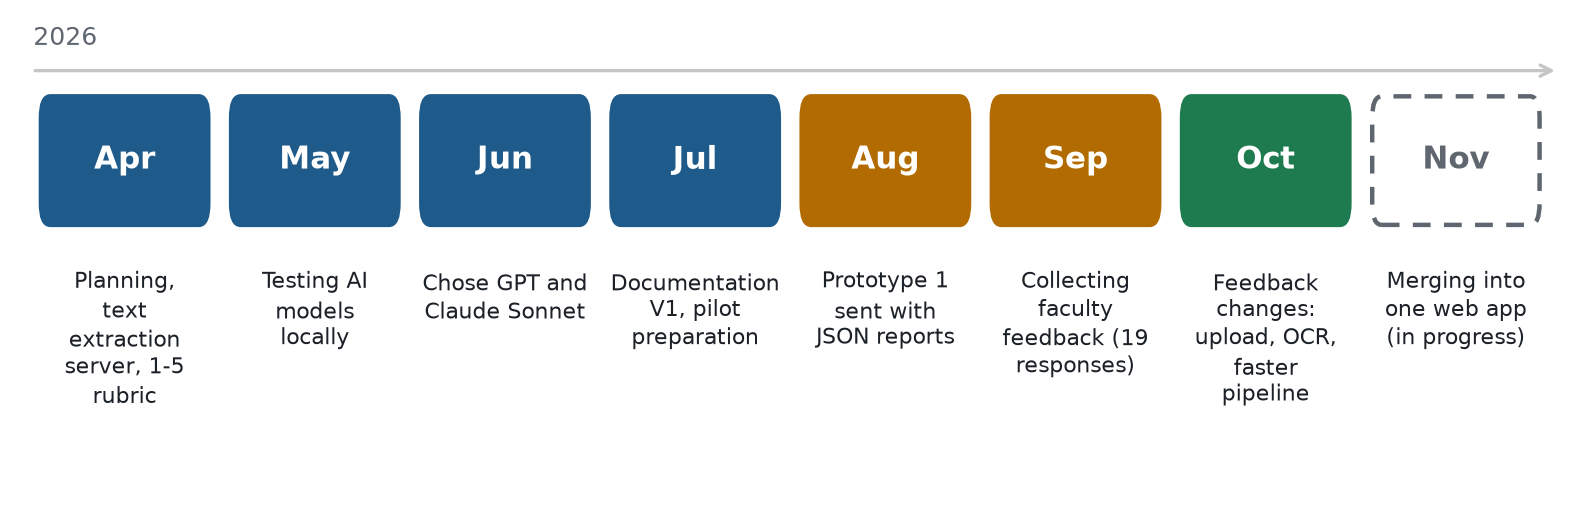
\includegraphics[keepaspectratio,alt={Project timeline by month, 2026}]{figures/timeline.png}}

\emph{Figure 1. The project month by month.}

{\def\LTcaptype{none} % do not increment counter
\begin{longtable}[]{@{}lll@{}}
\toprule\noalign{}
When (2026) & Phase & What happened \\
\midrule\noalign{}
\endhead
\bottomrule\noalign{}
\endlastfoot
April & Planning and text extraction & Architecture, data format and themes
planned. April 13: first version of the text extraction server (FastAPI, Word
and PDF). April 23: rubric meeting; the scale moved from 0 to 4 to \textbf{1 to
5} so a high score always means positive and no instructor sees a zero, Pace and
Workload were separated, and themes were merged or split into the final
\textbf{12 topics}. \\
May & Testing AI models locally & Local language models and classifiers were run
and compared against human labels: Llama3, Gemma 3, Qwen, RoBERTa-large-MNLI and
DistilRoBERTa (Section 4.1). \\
June & Choosing the models & June 12: methodology guide (normalization,
retrieval of similar human-graded examples, evidence-based topic classification,
rubric scoring, quote grounding, summaries). After trials on real evaluation
files, the hosted models \textbf{GPT (\texttt{gpt-5.6-terra})} and
\textbf{Claude Sonnet} were chosen; local Qwen stayed available for the research
team. June 24: first platform manual. \\
July & Documentation V1 and pilot preparation & July 16: \textbf{Documentation
V1} (five engineering pillars, two prompts per comment, confidence thresholds).
Reports generated for the pilot instructors and the Professor Portal
prepared. \\
August & Prototype 1 sent & \textbf{Prototype 1} went out: each pilot instructor
received a JSON report through Google Drive and opened it in the Professor
Portal, with a user manual and a feedback form. First responses on August 6. \\
September & Collecting feedback & Responses kept arriving until September 29:
\textbf{19 in total} (Section 4.3). \\
October & Improving from the feedback & Interface changes requested by
instructors, including \textbf{drag-and-drop upload}; "ignore comments" with
score recalculation and JSON export in the portal. \textbf{Text extraction (OCR)
fixed} and the \textbf{analysis pipeline improved} to cut the time to process a
document: whole answers with their questions, one structured call per answer,
parallel and cached calls, plus an evaluation harness and automated tests
(Section 4.2). \\
November & Merging into one web app (in progress) & Work under way to merge the
analysis pipeline and the portal into one application with instructor accounts,
AI budgets and private reports (Section 3.2). Cost estimate for a year of use
prepared (Section 4.4). Claude Sonnet dropped so that one provider handles cost
tracking and personal API keys. \\
\end{longtable}
}

\section{3. What changed and why}\label{3-what-changed-and-why}

\pandocbounded{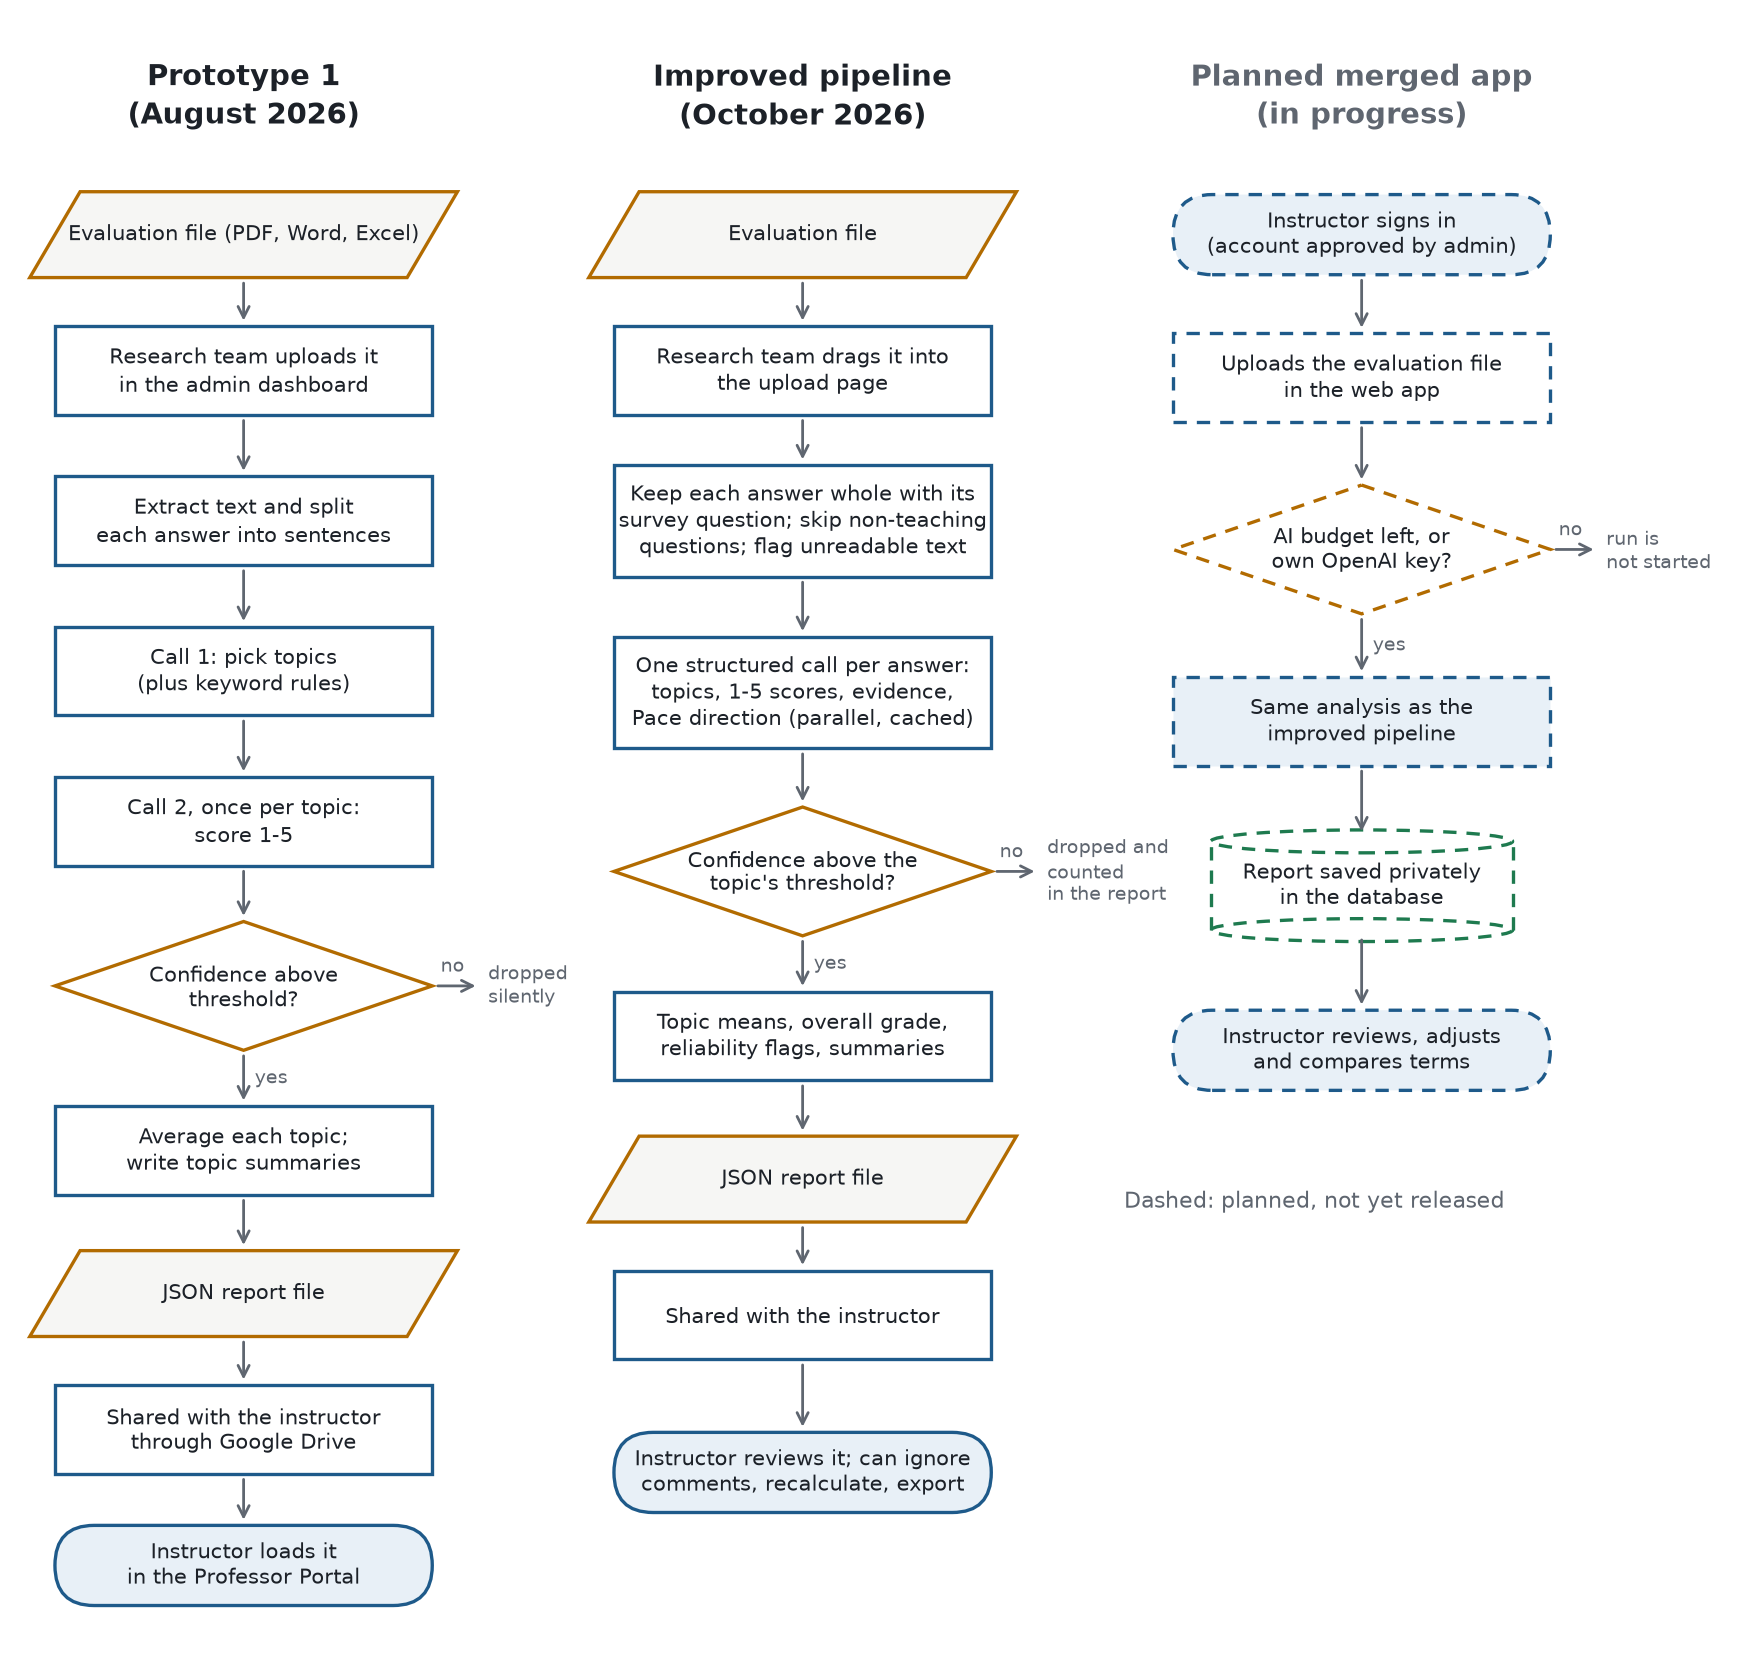
\includegraphics[keepaspectratio,alt={How an evaluation file becomes a report, in three stages}]{figures/flowchart.png}}

\emph{Figure 2. Flowchart of how an evaluation file becomes a report: in
prototype 1 (left), with the improved pipeline of October (middle), and in the
merged app being developed (right, dashed). Parallelograms are files, rectangles
are steps, diamonds are decisions, rounded boxes are where a person starts or
finishes, and the cylinder is the database.}

\subsection{3.1 From V1\textquotesingle s five pillars to the October
pipeline}\label{31-from-v1s-five-pillars-to-the-october-pipeline}

{\def\LTcaptype{none} % do not increment counter
\begin{longtable}[]{@{}llll@{}}
\toprule\noalign{}
V1 pillar (July 2026) & What it did in prototype 1 & What it does after October
& Why it changed \\
\midrule\noalign{}
\endhead
\bottomrule\noalign{}
\endlastfoot
1. Configuration and rules & Local Qwen model or a hosted model; per-topic
confidence thresholds (0.35 to 0.45); keyword hints that forced extra topics. &
Hosted model by default with a provider-enforced JSON schema; local Qwen kept
for the research team. Thresholds kept (Section 6). Keyword forcing
\textbf{removed}. & Keyword rules added topics the model then had to reject.
Schema enforcement removed malformed answers. \\
2. Data preparation and RAG & Cleaned text; split answers into
\textbf{sentences}; retrieved similar human-labelled examples. & Keeps each
\textbf{answer whole} with its survey question; skips answers to questions about
the student rather than the teaching; still retrieves examples (2 for topics, 1
for scoring) when the labelled files are present. & Splitting turned one answer
into many "comments" (one file: 410 fragments for 123 real answers) and made
fragments hard to interpret. Answers to non-teaching questions filled the
"Other" bin (about 25 \% of comments). \\
3. Categorization engine (prompt 1) & One call to pick topics. & Merged into a
single structured call. & Two calls per topic cost time and money and gave lower
accuracy (Section 4.2). \\
4. Scoring engine (prompt 2) & One more call per assigned topic. & The same call
returns, per topic, a 1 to 5 score, confidence, evidence quote and, for Pace,
the direction (too fast, too slow, about right). & As above. Pace previously
used a non-monotonic code (1 = too fast, 2 = too slow, ...), so its average was
meaningless; it now runs from 1 (serious problem) to 5 (well paced) with a
separate direction. \\
5. Main loop and export & Sequential calls; JSON and CSV export. & Up to 8
parallel calls (2 for the local model); answers cached so an unchanged re-run is
free; every dropped result and model error is counted in the report. & A large
file took up to 78 minutes; silent drops hid how much of a report rested on
uncertain results. \\
\end{longtable}
}

\subsection{3.2 Where the project is heading: one web application (in
progress)}\label{32-where-the-project-is-heading-one-web-application-in-progress}

Prototype 1 depended on the research team for every step. The merged application
is being built so instructors can do the whole process themselves. The table
compares prototype 1 with the goals of the merge; none of these features has
been released yet.

{\def\LTcaptype{none} % do not increment counter
\begin{longtable}[]{@{}ll@{}}
\toprule\noalign{}
Prototype 1 & Goal of the merged app \\
\midrule\noalign{}
\endhead
\bottomrule\noalign{}
\endlastfoot
The research team uploads each file and sends the instructor a JSON report
through Google Drive. & Instructors sign in, upload their own file, follow its
progress, and find the report in their account. \\
The instructor loads a file into the portal; reports are not stored. & Reports
are stored on the server, and each one can be opened only by the account that
created it. \\
No personal accounts. & Registration with administrator approval, password
rules, and lock-out after repeated failed sign-ins. \\
All AI use on the lab\textquotesingle s key, not tracked per person. & Every run
records its tokens and cost. The administrator gives each instructor lab credit
with a yearly dollar cap, lab credit without a cap, or the option to use their
own OpenAI key, stored encrypted. \\
One report at a time. & Comparison of two or more reports of the same course
across terms. \\
A separate PDF manual. & A built-in guide shown on first sign-in. \\
\end{longtable}
}

\section{4. Results}\label{4-results}

\subsection{4.1 Choosing a model (May to June
2026)}\label{41-choosing-a-model-may-to-june-2026}

The local comparison measured each approach against human labels. Topic
classification was measured on the benchmark comments that could be matched to
the human-labelled file (27 of 29); sentiment scoring on 195 human-scored
comment-topic pairs.

{\def\LTcaptype{none} % do not increment counter
\begin{longtable}[]{@{}lllllll@{}}
\toprule\noalign{}
Model & Topic micro F1 & Topic macro F1 & Exact topic set & Score exact & Score
within 1 & Score MAE \\
\midrule\noalign{}
\endhead
\bottomrule\noalign{}
\endlastfoot
Llama3 (local LLM) & 55.6 \% & 42.4 \% & 14.8 \% & 63.6 \% & 91.8 \% & 0.46 \\
Gemma 3 (local LLM) & 52.2 \% & 45.4 \% & 25.9 \% & 53.3 \% & 88.7 \% & 0.59 \\
RoBERTa-large-MNLI & 35.8 \% & 29.1 \% & 0.0 \% & 51.3 \% & 86.7 \% & 0.63 \\
DistilRoBERTa & 17.8 \% & 15.6 \% & 3.7 \% & 59.0 \% & 87.7 \% & 0.62 \\
Always predict 5 (baseline) & & & & 63.6 \% & 88.7 \% & 0.53 \\
\end{longtable}
}

\emph{Source: \texttt{NLP/results/topic\_model\_comparison.csv} and
\texttt{NLP/results/sentiment\_model\_comparison.csv}.}

Two findings shaped the next steps. First, zero-shot transformer classifiers
could not assign the twelve topics reliably, so the project committed to large
language models; the trials on real files in June then led to the hosted models.
Second, course evaluations are skewed positive: a constant prediction of 5
already matches 63.6 \% of human scores, so exact-match accuracy alone is a weak
measure. Later evaluations therefore also report the mean absolute error (MAE)
and agreement on positive or negative sentiment.

\subsection{4.2 Improving the pipeline (October
2026)}\label{42-improving-the-pipeline-october-2026}

The October work found that most errors came from what the model was given
rather than from the model itself. After the changes in Section 3.1 the pipeline
was measured again on the same 88 human-labelled comments with the same model
(\texttt{gpt-5.6-terra}, retrieval examples on).

\pandocbounded{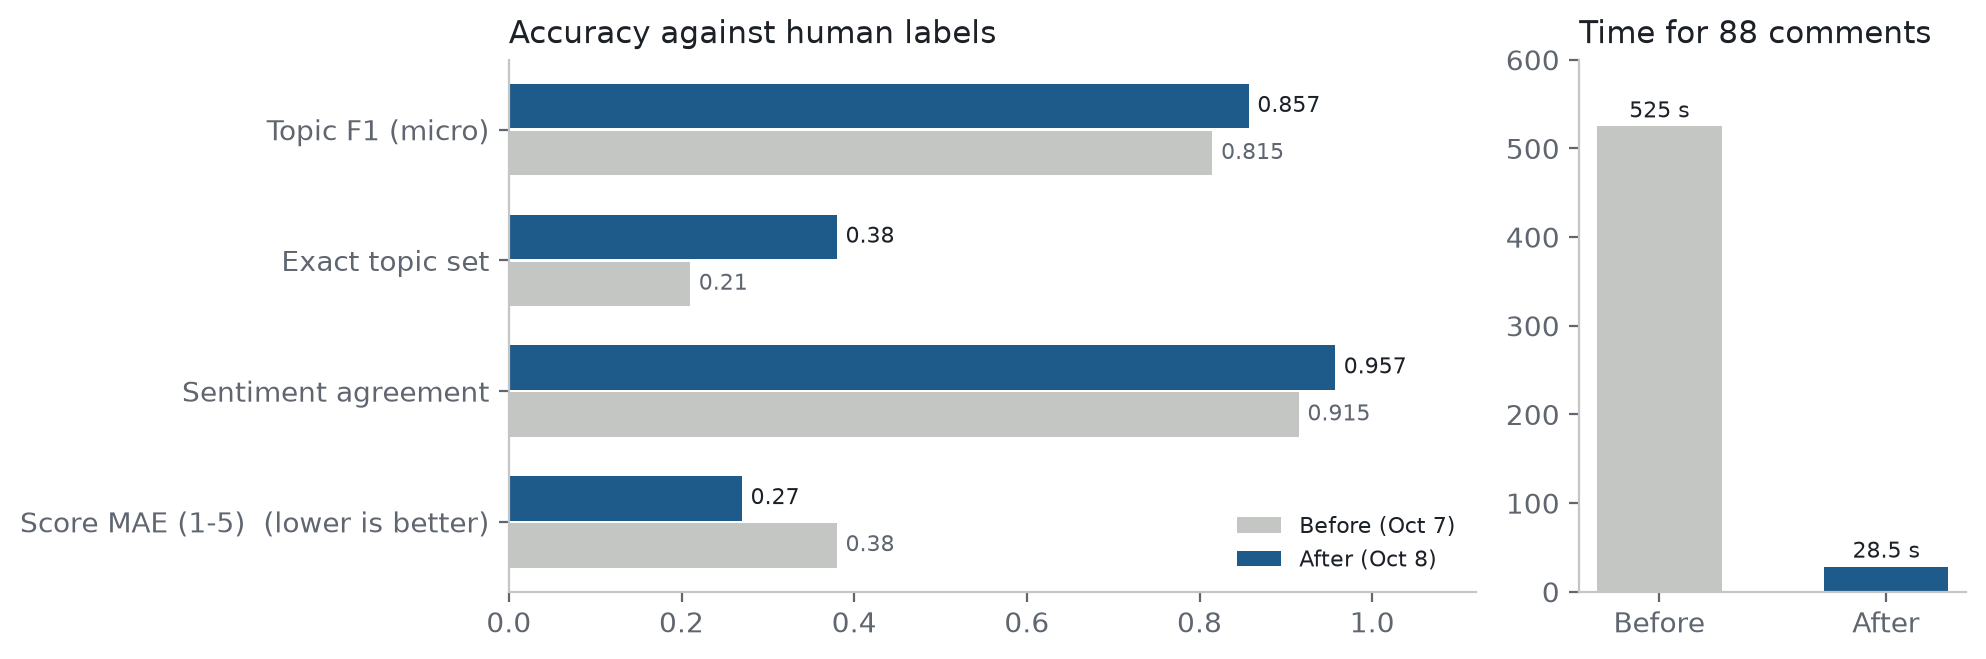
\includegraphics[keepaspectratio,alt={Accuracy and runtime before and after the pipeline improvements}]{figures/results.png}}

\emph{Figure 3. Agreement with human labels and processing time before and after
the pipeline improvements (measured October 7 and 8).}

{\def\LTcaptype{none} % do not increment counter
\begin{longtable}[]{@{}lll@{}}
\toprule\noalign{}
Measure (88 human-labelled comments) & Before & After \\
\midrule\noalign{}
\endhead
\bottomrule\noalign{}
\endlastfoot
Topic micro F1 & 0.815 & 0.857 \\
Topic macro F1 & & 0.741 \\
Comments with exactly the right set of topics & 21 \% & 38 \% \\
Score MAE on the 1 to 5 scale & 0.38 & 0.27 \\
Scores within 1 point of the human score & & 100 \% \\
Positive or negative agreement with humans & 91.5 \% & 95.7 \% \\
Time to process the 88 comments & 525 s & 28.5 s \\
\end{longtable}
}

\emph{Sources: \texttt{docs/Backend\_Improvements\_Report.pdf}; "after" details
from \texttt{NLP/eval\_runs/20261008\_131258\_openai/summary.json} (prompt
version 2026-10-08.4: topic metrics on 29 matched comments, score metrics on 157
comment-topic pairs).}

Per-topic F1 with the improved pipeline ranged from 1.0 (communication and
availability) and 0.96 (learning resources) down to 0.50 (inclusivity) and 0.0
(grading and feedback). With only 29 comments in the topic benchmark, the
weakest topics rest on very few labelled examples; a larger labelled set is a
main item of future work (Section 10).

On three real files the improvements changed what reached the model and how long
it took:

{\def\LTcaptype{none} % do not increment counter
\begin{longtable}[]{@{}llll@{}}
\toprule\noalign{}
File & Units sent to the model & Share left uncategorized & Processing time \\
\midrule\noalign{}
\endhead
\bottomrule\noalign{}
\endlastfoot
Large spreadsheet export & 410 fragments, now 123 whole answers & 25 \% to 5 \%
& 23.5 min to 52 s \\
PDF report & 34 to 50 answers & 24 \% to 8 \% & 97 s to 14 s \\
Converted Excel report & 32 fragments, now 16 answers & 9 \% to 0 \% & 118 s to
8 s \\
\end{longtable}
}

\emph{Source: \texttt{docs/Backend\_Improvements\_Report.pdf}.} Overall scores
moved slightly (for example 3.62 to 3.97) because long answers are no longer
counted several times. Pace averages from prototype 1 are not comparable with
later ones because the Pace rubric was corrected.

\subsection{4.3 What instructors said about prototype 1 (August to September
2026)}\label{43-what-instructors-said-about-prototype-1-august-to-september-2026}

Pilot instructors completed a feedback form after receiving their report: 19
responses between August 6 and September 29, 2026. Items used a 1 (strongly
disagree) to 5 (strongly agree) scale.

\pandocbounded{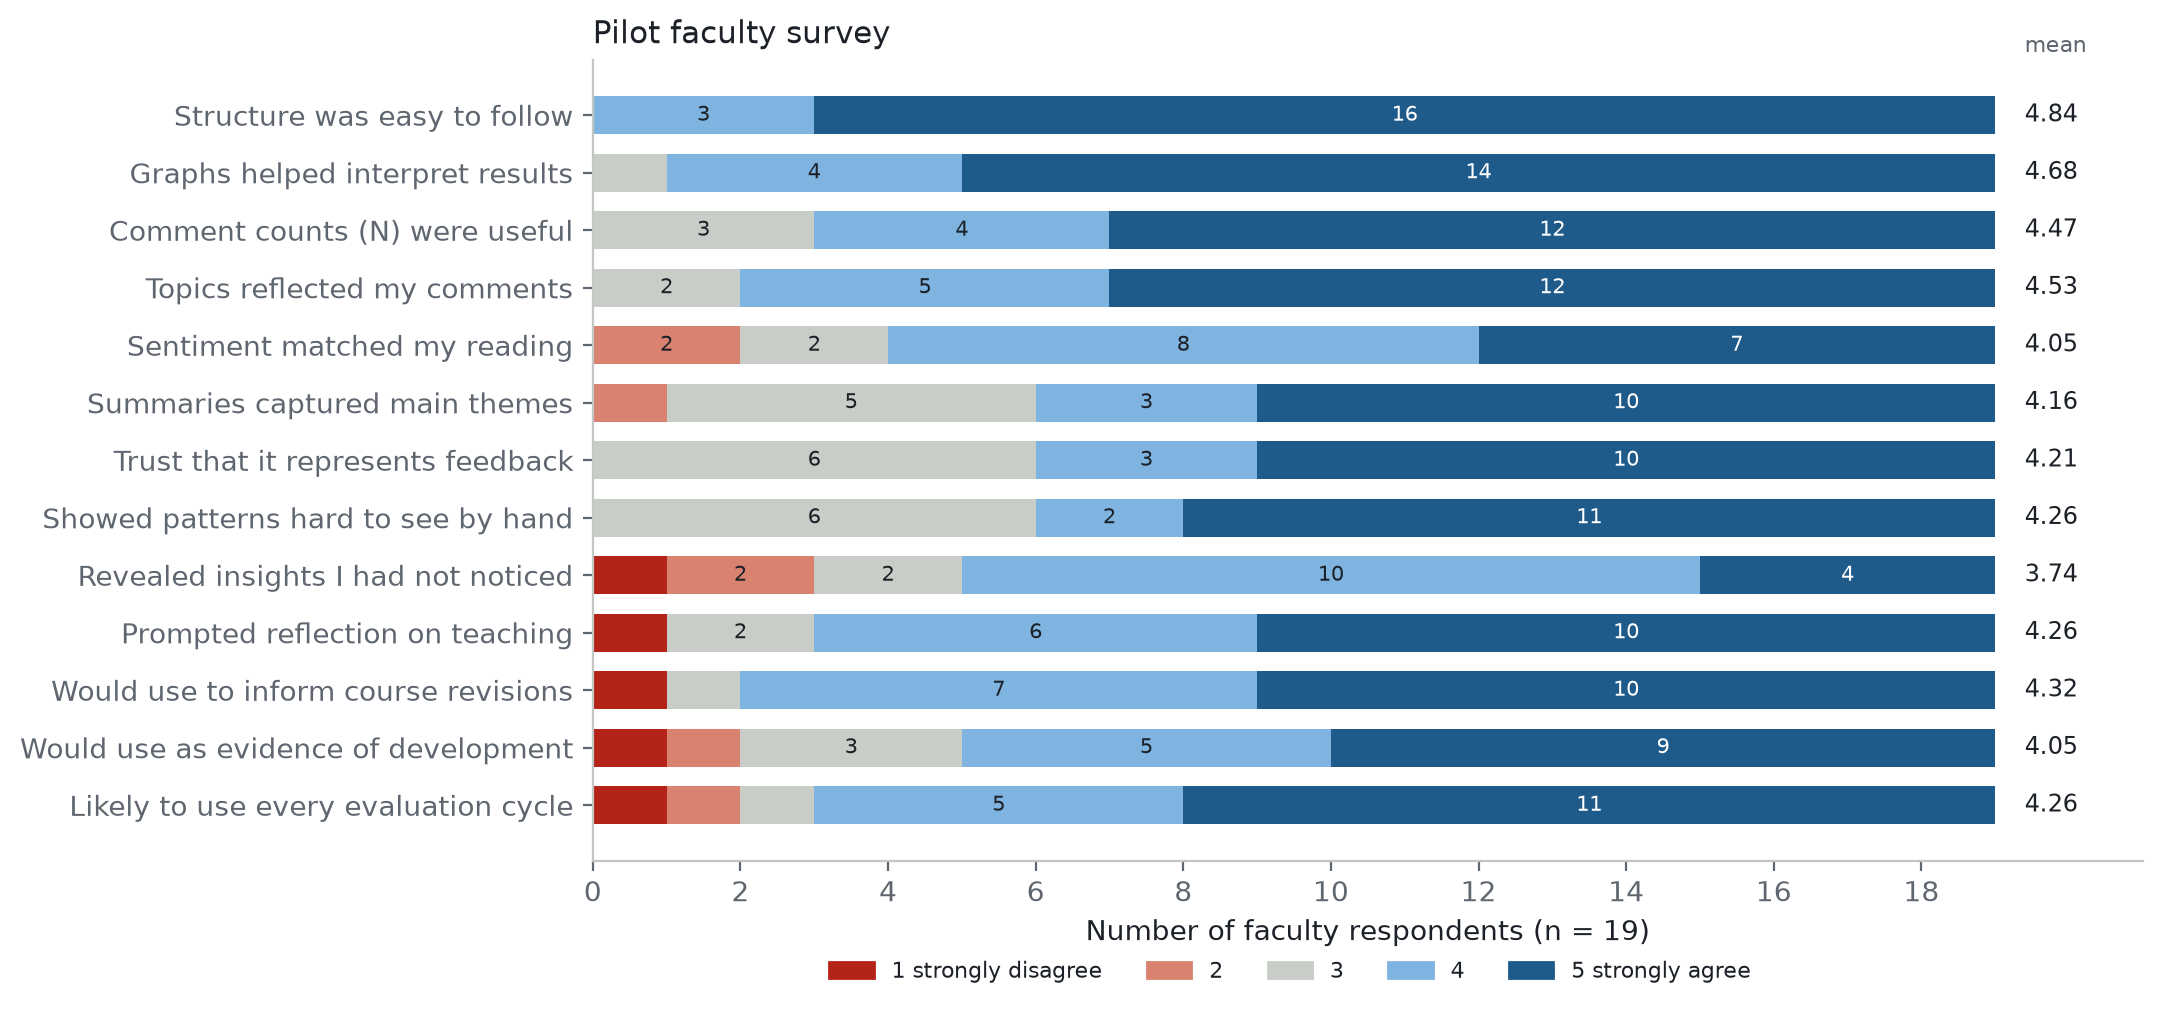
\includegraphics[keepaspectratio,alt={Pilot faculty survey}]{figures/pilot_survey.png}}

\emph{Figure 4. Responses to the prototype 1 feedback form (n = 19). Only
aggregate counts are shown.}

\begin{itemize}
\tightlist
\item
  \textbf{Usability was rated highest.} The structure was easy to follow (mean
  4.84), the graphs helped interpret the results (4.68) and the comment counts
  were useful (4.47).
\item
  \textbf{Accuracy was rated well, with room to improve.} The topics reflected
  the comments (4.53); the summaries captured the main themes (4.16); the
  sentiment matched the instructor\textquotesingle s own reading (4.05); and
  respondents trusted that the analysis represents their
  students\textquotesingle{} feedback (4.21). Fifteen of 19 called the tone of
  the analysis "about right", three "too critical" and one "too positive".
\item
  \textbf{New insight was rated lowest.} "Revealed insights I had not noticed"
  averaged 3.74, the only item below 4. This suggests the tool mainly organizes
  and confirms what attentive instructors already sense, and its value lies in
  the time saved and the evidence it collects.
\item
  \textbf{Intended use was strong.} Instructors would use it to inform course
  revisions (4.32) and after every evaluation cycle (4.26), and somewhat less as
  evidence of teaching effectiveness (4.05).
\end{itemize}

\emph{Source: aggregate answer counts from the prototype 1 feedback form export
(19 responses; not in the repository).}

The feedback set the October work: easier uploading (drag and drop), more
reliable text extraction, faster processing, the ability to leave out comments
that do not apply and recalculate, and export. Requests that need accounts and
stored reports, such as comparing courses or terms, moved into the merged
application.

\subsection{4.4 Cost estimate for the merged
app}\label{44-cost-estimate-for-the-merged-app}

For the merged application, where instructors will run their own analyses, a
year of use was estimated from offline prompt measurements: about 3,000 input
tokens per answer (about 2,500 of them the fixed rubrics) and about 250 output
tokens. An average file has 186 answers, of which about 153 are analysed. At 250
files a year this comes to roughly \textbf{\$230 to \$500} of OpenAI usage,
depending on prompt caching and list price, so a typical file costs a few cents
to about a dollar. \emph{Source: \texttt{docs/Phase0\_Purchase\_Estimate.pdf}.}
The pipeline now records the tokens and cost of every run, so the estimate can
be replaced by measured figures once the app is in use.

\section{5. How the analysis works now}\label{5-how-the-analysis-works-now}

This chapter replaces V1\textquotesingle s "Core functional pillars" and
describes the improved pipeline from October 2026.

\subsection{Step 1: Extraction}\label{step-1-extraction}

The extraction server reads PDF, Excel, CSV and Word exports. It keeps each
student answer whole, joins lines that the export had wrapped, records the
survey question each answer responds to, and removes list bullets and stray
encoding characters. Survey boilerplate, rating rows and unreadable PDF text are
filtered with rules and a small TF-IDF plus linear SVM classifier. When a
PDF\textquotesingle s text is mostly not real words (some fonts store letters as
symbols), the report says so and asks for an Excel or CSV export instead of
analysing gibberish. Multiple-choice rating tables in Excel and CSV exports are
read into their own section with counts, mean and full distribution; PDF rating
tables are not read yet.

\subsection{Step 2: Preparation}\label{step-2-preparation}

Exact duplicate answers are removed. Answers to questions about the student
rather than the teaching ("Did you feel prepared by prior coursework?") go
straight to "Other" without an AI call and are counted in the report.

\subsection{Step 3: One structured analysis per
answer}\label{step-3-one-structured-analysis-per-answer}

Each answer is sent once, with its survey question, the twelve topic definitions
and the 1 to 5 rubric. When the human-labelled files are present, the most
similar labelled examples are added for calibration. The provider enforces a
JSON schema, so the reply always parses. For every topic the answer actually
discusses, the reply gives:

\begin{itemize}
\tightlist
\item
  the topic and the model\textquotesingle s confidence;
\item
  a 1 to 5 score on that topic\textquotesingle s rubric;
\item
  an evidence quote from the answer;
\item
  for Pace, whether the course felt too fast, too slow or about right.
\end{itemize}

Generic comments with no specific topic ("Best professor ever!") receive a
separate general-sentiment score instead.

The twelve topics are: course organization and structure; pace; workload;
student engagement and participation; clarity of explanations; effectiveness of
assignments; classroom atmosphere; instructor\textquotesingle s communication
and availability; inclusivity and sense of belonging; assessment; grading and
feedback; learning resources and materials.

\subsection{Step 4: Filtering}\label{step-4-filtering}

A topic score is dropped when the model\textquotesingle s confidence is below
that topic\textquotesingle s threshold: 0.45 for Assessment and Workload, 0.40
for Pace and Course organization, 0.35 otherwise. Stricter topics need stronger
evidence because their vocabulary overlaps with others. Every drop and every
model error is counted in the report rather than silently discarded.

\subsection{Step 5: Aggregation and
summaries}\label{step-5-aggregation-and-summaries}

Topic averages, the overall score and reliability flags are computed (Section
6). A final call per topic writes a one-sentence summary of what students said
about it. Calls run in parallel and are cached, so re-running an unchanged file
costs nothing.

\section{6. Dashboard metrics explained}\label{6-dashboard-metrics-explained}

This chapter replaces V1\textquotesingle s chapter 3. What V1 said about
averages and multi-topic answers still holds; the changes are in how the overall
grade is formed and in the reliability flags.

\begin{itemize}
\tightlist
\item
  \textbf{Topic score.} The mean of the valid 1 to 5 scores for that topic.
  Answers that mention a topic without evaluating it ("Labs") still appear on
  the topic for context but are not part of the average, so the number of
  comments on a topic and the number of scored comments can differ, by design.
\item
  \textbf{Overall grade.} The mean, over answers, of each
  answer\textquotesingle s average topic score. A long answer touching five
  topics counts once, like a short one, and cannot outweigh it.
\item
  \textbf{General sentiment.} Generic praise or criticism is reported separately
  and never changes the overall grade.
\item
  \textbf{Multi-topic answers.} Each topic gets its own independent score. "The
  pace was too fast, but the homework was great" produces a low Pace score and a
  high assignments score, not one muddled average.
\item
  \textbf{Pace direction.} Alongside its score, Pace reports how many answers
  said too fast, too slow or about right.
\item
  \textbf{Reliability flags.} Each topic carries one flag:

  \begin{itemize}
  \tightlist
  \item
    \emph{reliable}: five or more scored comments and no warnings;
  \item
    \emph{low sample}: fewer than five scored comments, so read it as
    directional evidence only;
  \item
    \emph{mixed confidence}: some scores rest on low model confidence (below
    0.35), so read the comments;
  \item
    \emph{needs review}: a model error was excluded;
  \item
    \emph{unscored}: no scored comments.
  \end{itemize}
\item
  \textbf{Ignoring comments.} An instructor can exclude comments that do not
  apply to a topic (for example, a remark about a different course). The topic
  and overall scores are recalculated with the same rules as the pipeline, and
  the excluded comments stay visible, marked as ignored.
\end{itemize}

\section{7. The website: prototype 1, October changes and the app in
development}\label{7-the-website-prototype-1-october-changes-and-the-app-in-development}

\pandocbounded{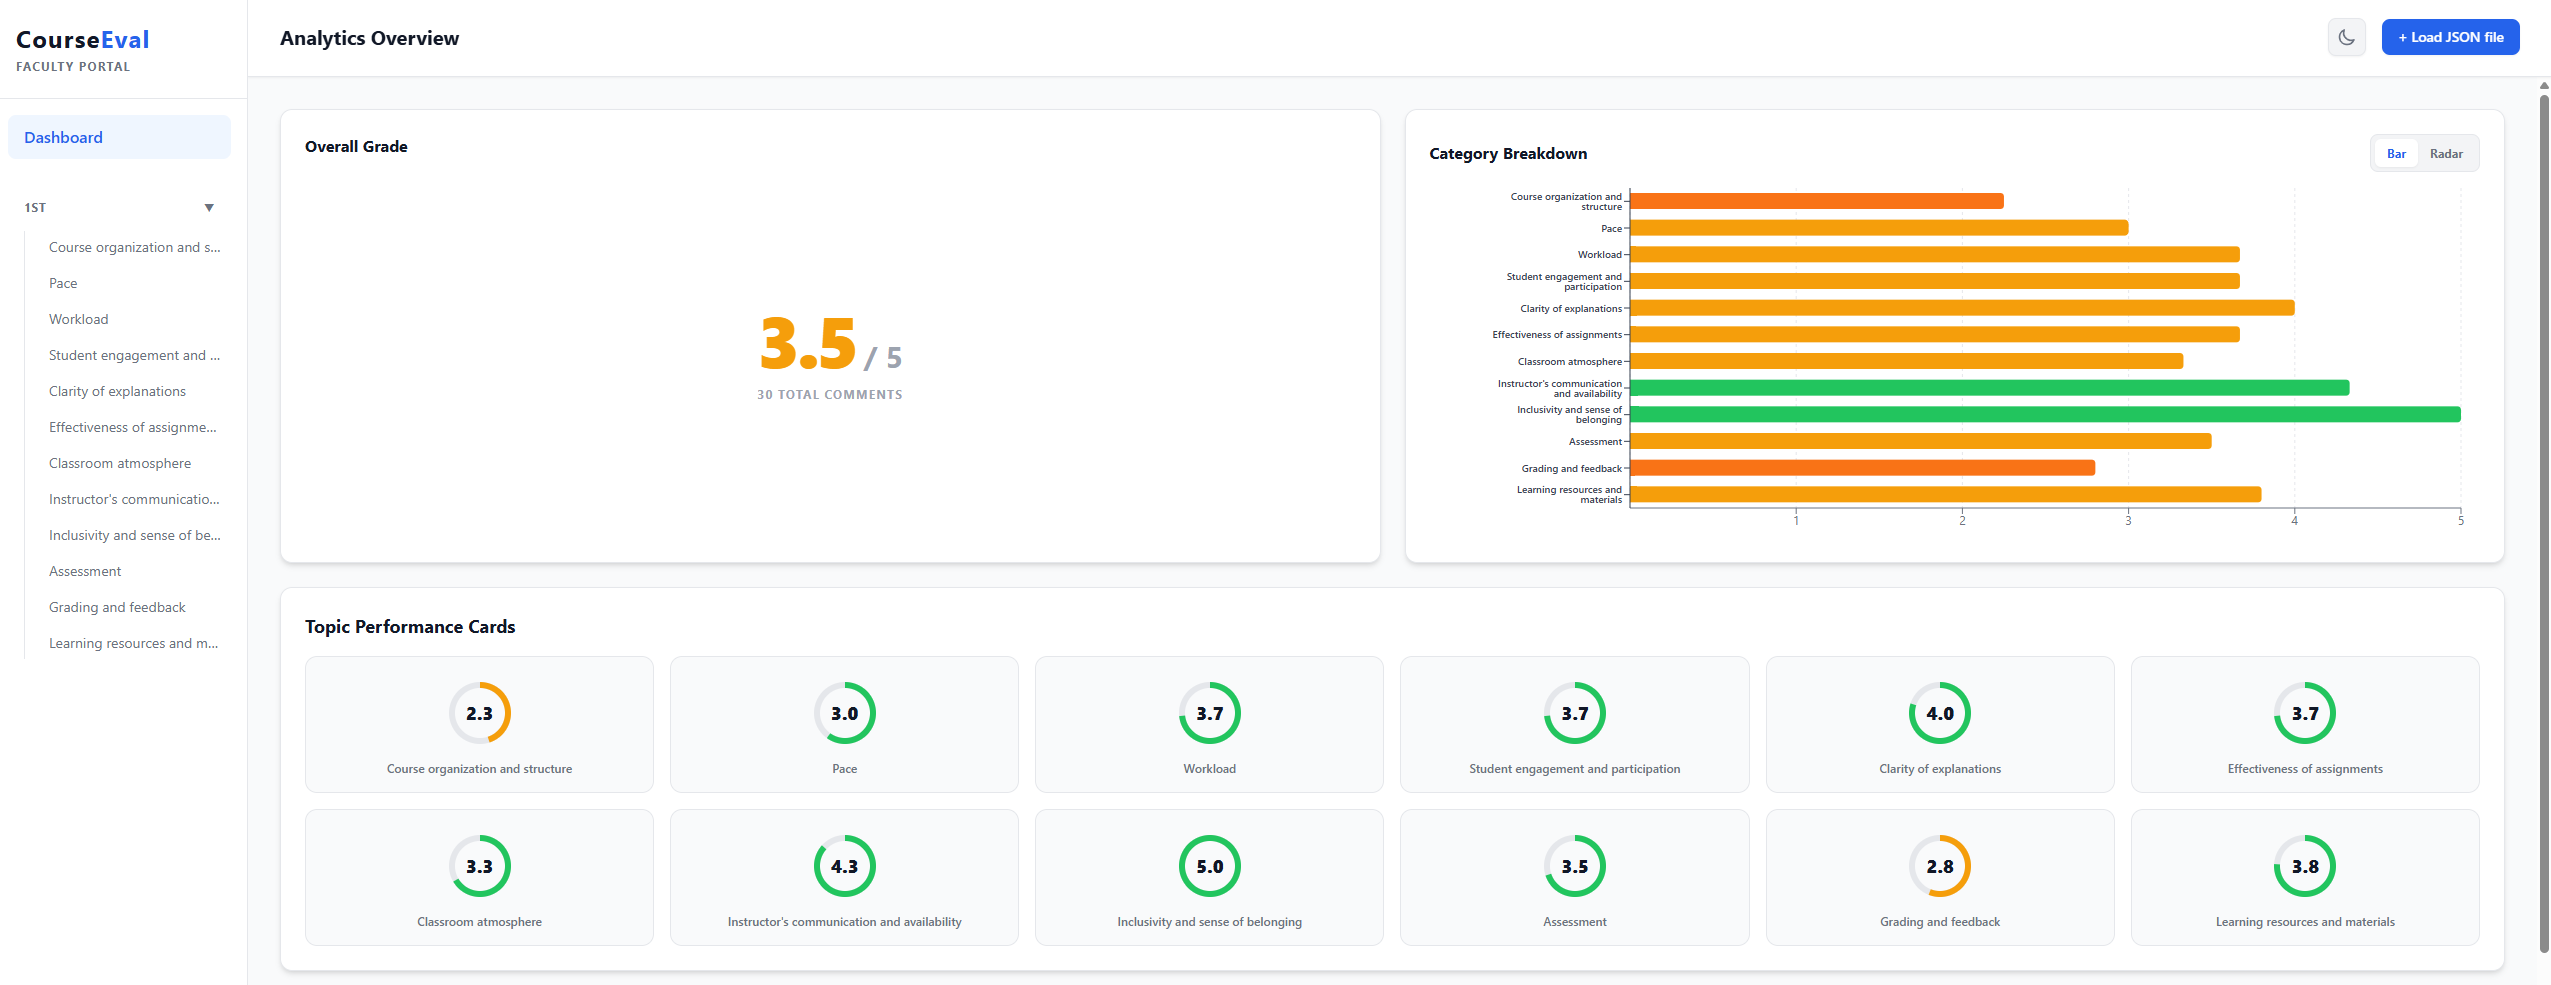
\includegraphics[keepaspectratio,alt={The Professor Portal in prototype 1}]{figures/then_portal.png}}

\emph{Figure 5. The Professor Portal in prototype 1: the instructor loaded the
JSON report shared by the research team. Shown above the comment list only;
course identity removed.}

\textbf{Prototype 1 (August).} Instructors downloaded their JSON report from a
shared Google Drive folder and loaded it into the Professor Portal. The portal
showed the overall grade, a category chart that switched between bar and radar,
a score card for each topic, a detailed view per topic with its comments and
summary, and a filterable comment list.

\textbf{After the feedback (October).} Uploading moved to drag and drop;
comments that do not apply can be ignored for a topic, the scores recalculated,
and the edited report exported; comment text is cleaned of stray symbols; and
reports arrive much faster because of the improved pipeline.

\textbf{The merged app (in development).} The goal is one site where
instructors:

\begin{enumerate}
\def\labelenumi{\arabic{enumi}.}
\tightlist
\item
  request an account and, once approved, are welcomed with a short guide;
\item
  upload an evaluation file and follow its progress;
\item
  read the report: overall grade, category chart, topic cards, a detail view per
  topic, and a searchable list of every analysed comment;
\item
  ignore comments and recalculate, and download the report;
\item
  compare two or more terms of the same course;
\item
  see the AI credit left for the year, or add their own OpenAI key.
\end{enumerate}

Its interface is still changing, so the figures below are placeholders until it
is finalized.

\pandocbounded{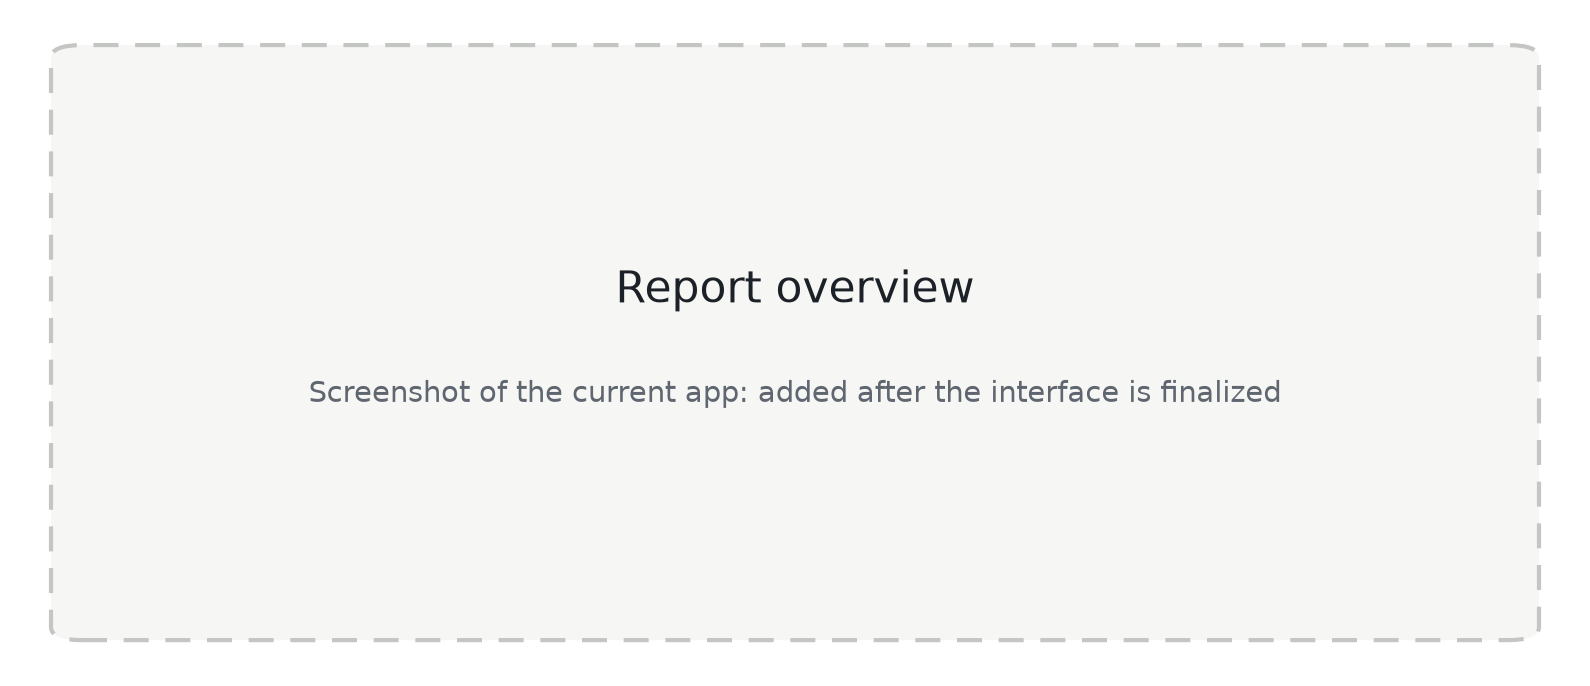
\includegraphics[keepaspectratio,alt={Report overview (placeholder)}]{figures/placeholder_overview.png}}

\emph{Figure 6. Placeholder for the report overview in the merged app.}

\pandocbounded{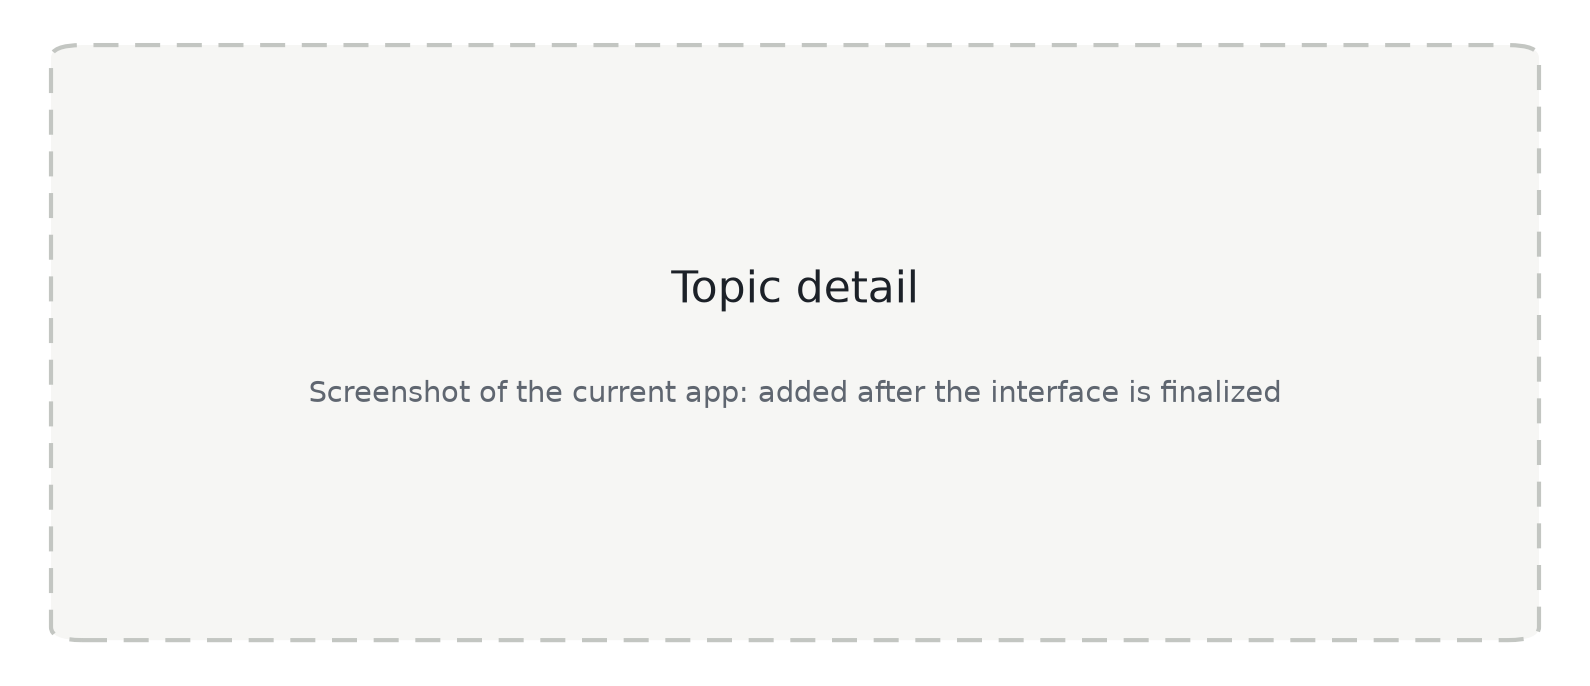
\includegraphics[keepaspectratio,alt={Topic detail (placeholder)}]{figures/placeholder_topic.png}}

\emph{Figure 7. Placeholder for the topic detail view in the merged app.}

\pandocbounded{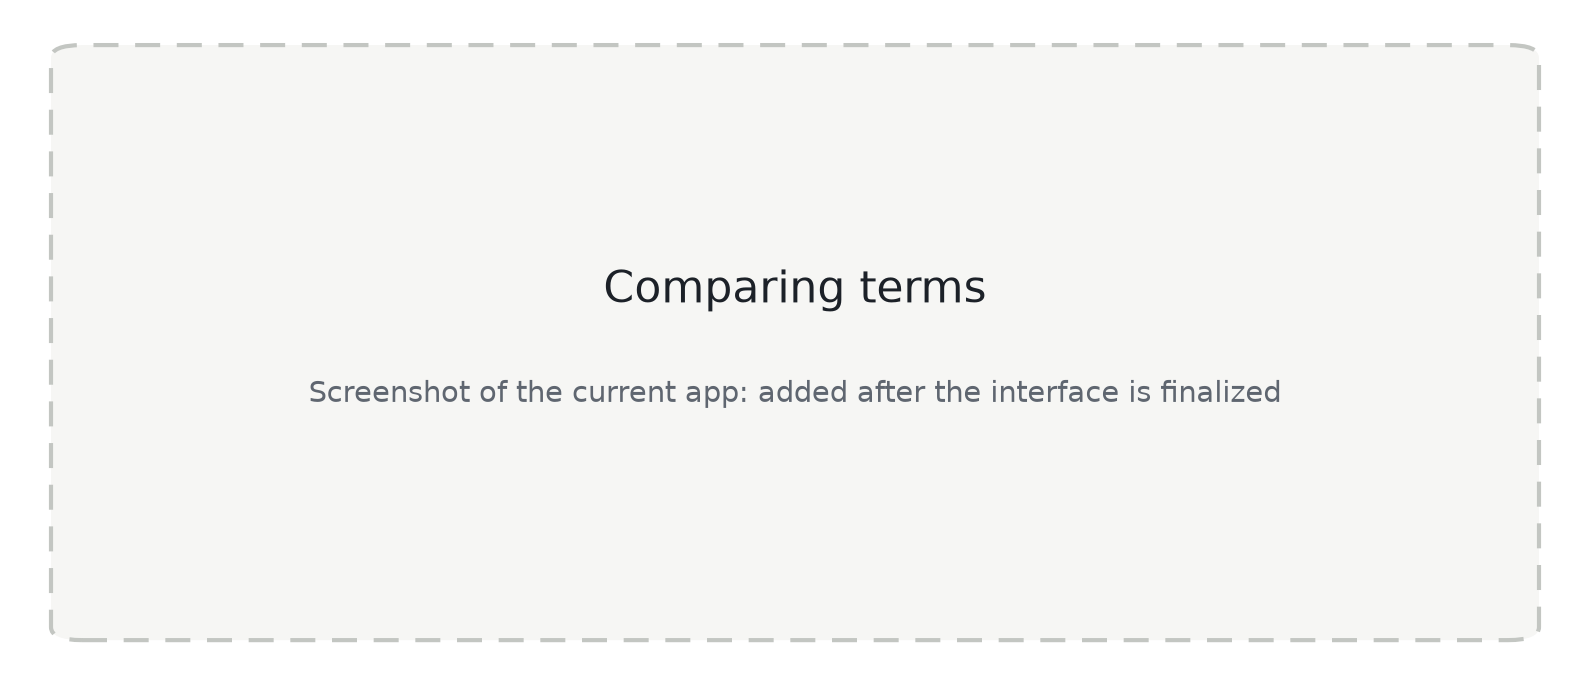
\includegraphics[keepaspectratio,alt={Comparing terms (placeholder)}]{figures/placeholder_compare.png}}

\emph{Figure 8. Placeholder for comparing terms in the merged app.}

\section{8. Evaluation method}\label{8-evaluation-method}

\begin{itemize}
\tightlist
\item
  \textbf{Ground truth.} Two human-labelled files: topic assignments for
  benchmark comments (\texttt{HUMAN\_CATEGORIZED\_OUTPUT.csv}) and topic-level
  scores with reasoning (\texttt{HUMAN\_SENTIMENT\_BASELINE.csv}).
\item
  \textbf{Topic metrics.} Micro and macro F1 over the twelve topics plus
  "Other", and the share of comments whose full topic set matches exactly.
\item
  \textbf{Score metrics.} MAE on the 1 to 5 scale; share of exact and within-1
  matches; agreement on positive (4 to 5) versus negative (1 to 2) sentiment;
  coverage (the share of human-scored pairs the model also scored).
\item
  \textbf{Harness.} \texttt{NLP/eval.py} runs the pipeline on the labelled
  comments and writes a summary per run to \texttt{NLP/eval\_runs/}. Every
  change in Section 3.1 was measured this way before it was kept.
\item
  \textbf{Automated tests.} Tests for the analysis pipeline and its API use a
  fake model, so they cost nothing and never touch student data; the merged app
  is being built with its own test suite.
\item
  \textbf{Limitations.} The labelled benchmark is small (88 comments; 29 for
  topic metrics) and comes from a small number of courses, so per-topic results
  for rare topics are unstable. The model is a commercial API whose behaviour
  can change between versions; each report records the model ID and prompt
  version. The pilot survey is self-reported by volunteers who had already
  received a report.
\end{itemize}

\section{9. Privacy, security and data
handling}\label{9-privacy-security-and-data-handling}

\textbf{In place today}

\begin{itemize}
\tightlist
\item
  \textbf{Who runs analyses.} Only the research team uploads evaluation files
  and runs the analysis.
\item
  \textbf{Server access.} The analysis server listens only on the local machine
  by default, accepts requests only from the admin dashboard and can require an
  access key. Uploaded file names are cleaned so they cannot reach other
  folders, and earlier reports are archived rather than overwritten.
\item
  \textbf{Sharing.} Each instructor receives only their own report.
\item
  \textbf{Student data in the repository.} None. Raw evaluations, generated
  reports, the human-labelled files and the model cache are excluded from
  version control. Figure 5 is cropped so no student text appears.
\item
  \textbf{Third-party processing.} Comments are sent to the hosted model for
  analysis unless the local model is chosen.
\end{itemize}

\textbf{Being built into the merged app}

\begin{itemize}
\tightlist
\item
  Reports visible only to the account that created them.
\item
  Instructor accounts with administrator approval, hashed passwords, password
  rules and lock-out after repeated failed sign-ins.
\item
  Personal API keys encrypted at rest, shown only as their last four characters,
  and never logged.
\item
  Per-instructor AI budgets, with every run\textquotesingle s cost recorded.
\item
  A database backed up nightly.
\end{itemize}

\section{10. Lessons learned and next
steps}\label{10-lessons-learned-and-next-steps}

\textbf{Lessons}

\begin{enumerate}
\def\labelenumi{\arabic{enumi}.}
\tightlist
\item
  \textbf{Fix the input before tuning the model.} The largest accuracy gains
  came from keeping answers whole and passing the survey question, not from
  changing models.
\item
  \textbf{Measure before keeping a change.} A small labelled benchmark and a
  repeatable harness turned design debates into measurements.
\item
  \textbf{Fewer, structured calls beat more calls.} One schema-enforced call per
  answer was faster, cheaper and more accurate than separate classification and
  scoring calls.
\item
  \textbf{Make uncertainty visible.} Instructors trusted the reports more when
  thin evidence was flagged rather than hidden.
\item
  \textbf{Pilot early.} Prototype 1 showed what instructors valued (clarity,
  charts, comment counts) and what they needed next (easier upload, speed,
  control over comments, comparison across terms).
\end{enumerate}

\textbf{Next steps}

\begin{itemize}
\tightlist
\item
  Finish, test and release the merged web application.
\item
  Enlarge and diversify the labelled benchmark, especially for rare topics, and
  measure inter-rater agreement.
\item
  Read rating tables from PDF exports.
\item
  Move hosting to a managed cloud provider once funding is confirmed.
\item
  Replace the cost estimate with measured cost per file.
\item
  Study whether instructors change their courses after using the reports (the
  pilot measured intent only).
\end{itemize}

\section{Appendix A. Commit timeline}\label{appendix-a-commit-timeline}

{\def\LTcaptype{none} % do not increment counter
\begin{longtable}[]{@{}ll@{}}
\toprule\noalign{}
Date (2026) & Change \\
\midrule\noalign{}
\endhead
\bottomrule\noalign{}
\endlastfoot
April 13 & FastAPI text extraction server with Word support; PDF extraction and
text sanitization \\
October 7 & Repository consolidated: extraction server, analysis pipeline and
API, admin dashboard, Professor Portal; ignore-comments mode with recalculation
and export \\
October 8 & Whole answers with questions and rating tables; single structured
analysis, parallel calls, cache, background jobs, evaluation harness \\
October 28 & Bullet symbols removed from comments in the portal \\
November & Merged web application in development \\
\end{longtable}
}

\section{Appendix B. Where things are}\label{appendix-b-where-things-are}

{\def\LTcaptype{none} % do not increment counter
\begin{longtable}[]{@{}ll@{}}
\toprule\noalign{}
Path & What it holds \\
\midrule\noalign{}
\endhead
\bottomrule\noalign{}
\endlastfoot
\texttt{OCR/} & Text extraction server \\
\texttt{NLP/main.py}, \texttt{NLP/data.py} & Analysis pipeline; topic
definitions and rubric \\
\texttt{NLP/eval.py}, \texttt{NLP/experiments.md} & Evaluation harness; model
comparison runbook \\
\texttt{ProfessorPortal/}, \texttt{dashboard/} & Professor Portal and admin
dashboard \\
\texttt{CourseEvalApp/} & Merged web application (in development) \\
\texttt{docs/documentation-v2/} & This document, its figures, and the LaTeX
version for Overleaf \\
\end{longtable}
}

\section{Appendix C. Glossary}\label{appendix-c-glossary}

\begin{itemize}
\tightlist
\item
  \textbf{F1 score.} Balance of precision (topics the model assigned that were
  right) and recall (right topics the model found). \emph{Micro} pools all
  decisions; \emph{macro} averages per topic, so rare topics count equally.
\item
  \textbf{MAE.} Mean absolute error: the average distance between the
  model\textquotesingle s score and the human score on the 1 to 5 scale.
\item
  \textbf{RAG.} Retrieval-augmented generation: adding similar human-labelled
  examples to the prompt.
\item
  \textbf{Structured output.} A reply the provider forces to follow a JSON
  schema, so it can always be read by the program.
\item
  \textbf{Prompt caching.} The provider\textquotesingle s discount for prompt
  text repeated exactly at the start of a request (here, the rubrics).
\end{itemize}

\end{document}
